\section{Correction to BBC-Small }\label{section:star_bbc}
The SDT trigger conditions imposed signal in RPs and veto on any signal in the same-side small BBC tiles, whereas signal in the opposite-side BBC-small was required by the offline event selection. A common BBC-small efficiency, $\epsilon_\textrm{BBC}$, was obtained as a function of each measured quantity using  PYTHIA 8 4C (SaS) embedded into Zerobias data. 
The efficiency was calculated  for events within fiducial region as follows:
\begin{equation}
\epsilon_\textrm{BBC}=\frac{\textrm{number of MC events satysfying the BBC-small selection criteria}}{\textrm{number of MC events}}
\end{equation}

\Cref{fig:bbcCorection_nch,fig:bbcCorection_pt,fig:bbcCorection_eta} show the fraction of generated true-level MC events, within the fiducial region of the measurement, in which the selection criteria on BBC-small signal and veto are fulfilled. The $\epsilon_\textrm{BBC}$  varies from about $90\%$ for events with $\xi$ within $0.02-0.05$ to about $65\%$ for events with $0.1<\xi<0.2$.

\begin{figure}[h!]
	%\vspace{-0.5cm}
	\centering
	\begin{subfigure}{.45\textwidth}
		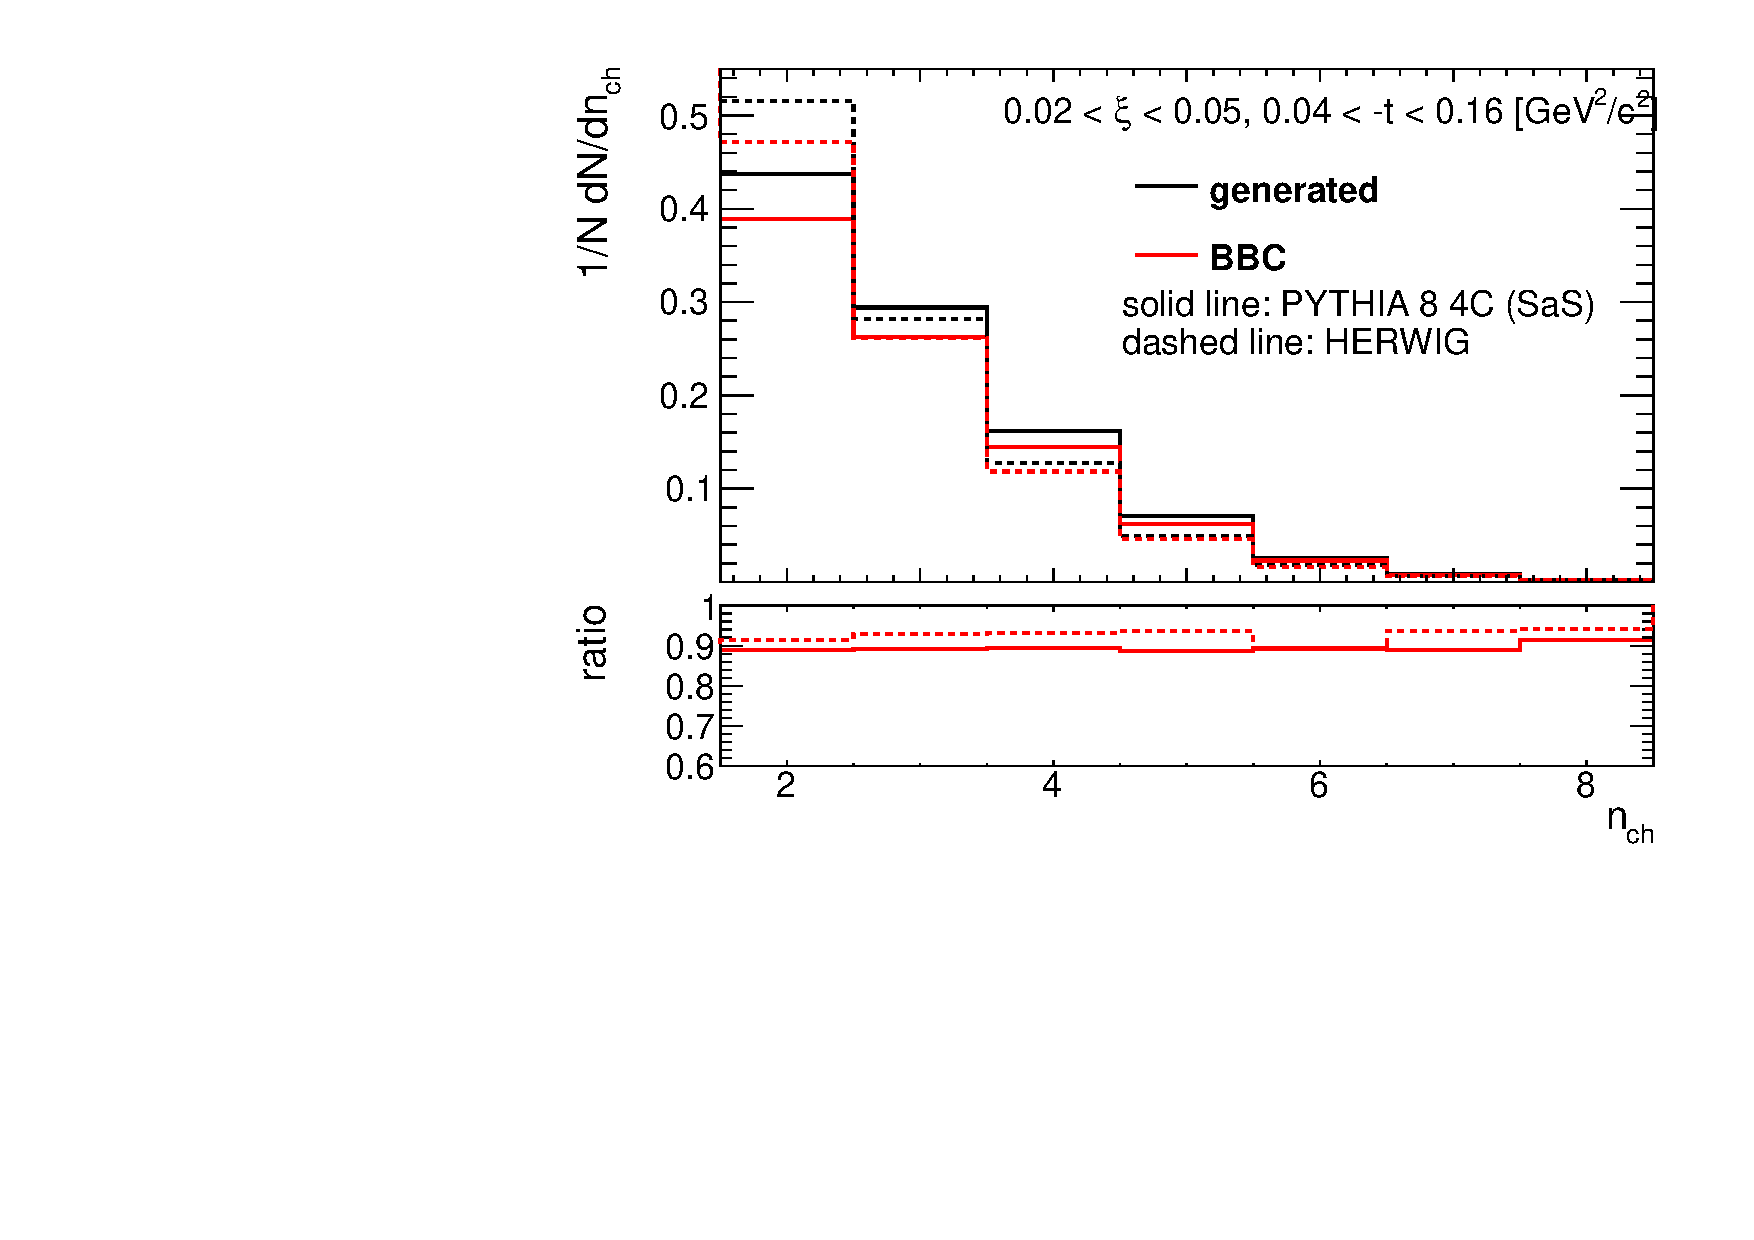
\includegraphics[width=\textwidth,page=1]{chapters/chrgSTAR/img/bbcCorrection/xi_bbc.pdf}
	\end{subfigure}
	\begin{subfigure}{.45\textwidth}
		\includegraphics[width=\textwidth,page=2]{chapters/chrgSTAR/img/bbcCorrection/xi_bbc.pdf}
	\end{subfigure}
	\begin{subfigure}{.45\textwidth}
		\includegraphics[width=\textwidth,page=3]{chapters/chrgSTAR/img/bbcCorrection/xi_bbc.pdf}
	\end{subfigure}
	\begin{minipage}{.45\textwidth}
		\caption{Number of true-level MC events which fulfill BBC-small selection criteria  as a function of $n_\textrm{ch}$ in three ranges of $\xi$. The fraction of such events is shown in the bottom pad.}
		\label{fig:bbcCorection_nch}
	\end{minipage}
	%\vspace{-0.5cm}
\end{figure}
\begin{figure}[h!]
	%\vspace{-0.5cm}
	\centering
	\begin{subfigure}{.45\textwidth}
		\includegraphics[width=\textwidth,page=5]{chapters/chrgSTAR/img/bbcCorrection/xi_bbc.pdf}
	\end{subfigure}
	\begin{subfigure}{.45\textwidth}
		\includegraphics[width=\textwidth,page=6]{chapters/chrgSTAR/img/bbcCorrection/xi_bbc.pdf}
	\end{subfigure}
	\begin{subfigure}{.45\textwidth}
		\includegraphics[width=\textwidth,page=7]{chapters/chrgSTAR/img/bbcCorrection/xi_bbc.pdf}
	\end{subfigure}
	\begin{minipage}{.45\textwidth}
		\caption{Number of true-level MC events which fulfill BBC-small selection criteria  as a function of $p_\textrm{T}$ in three ranges of $\xi$. The fraction of such events is shown in the bottom pad.}
		\label{fig:bbcCorection_pt}
	\end{minipage}
	%\vspace{-1.cm}
\end{figure}

\begin{figure}[h!]
	\centering
	\begin{subfigure}{.45\textwidth}
		\includegraphics[width=\textwidth,page=9]{chapters/chrgSTAR/img/bbcCorrection/xi_bbc.pdf}
	\end{subfigure}
	\begin{subfigure}{.45\textwidth}
		\includegraphics[width=\textwidth,page=10]{chapters/chrgSTAR/img/bbcCorrection/xi_bbc.pdf}
	\end{subfigure}
	\begin{subfigure}{.45\textwidth}
		\includegraphics[width=\textwidth,page=11]{chapters/chrgSTAR/img/bbcCorrection/xi_bbc.pdf}
	\end{subfigure}
	\begin{minipage}{.45\textwidth}
		\caption{Number of true-level MC events which fulfill BBC-small selection criteria  as a function of $\bar{\eta}$ in three ranges of $\xi$. The fraction of such events is shown in the bottom pad.}
		\label{fig:bbcCorection_eta}
	\end{minipage}
	
\end{figure}
%\FloatBarrier

%\subsubsection{Systematic Uncertainty}
When the data is corrected for BBC-small efficiency, there is an assumption that the MC used in the analysis, PYTHIA~8~4C~(SaS), provides correct correlation between the true value of $\xi$ and forward particles produced in the BBC acceptance region.  The uncertainty related to this correction is  estimated by using HERWIG~MC sample, where the hadronisation model is different from that used in PYTHIA~8. Figure~\ref{fig:bbcCorection_syst} shows the PYTHIA~8  prediction on BBC efficiency  divided by the HERWIG prediction in three ranges of $\xi$. The deviations between these two models are of the order of $2\%$ at $0.05<\xi<0.1$ and about $10\%$ for  other two $\xi$ regions. The difference between these two hadronisation models is used as systematic uncertainty.

\begin{figure}[h!]
	\centering
	\begin{subfigure}{.45\textwidth}
		\includegraphics[width=\textwidth,page=4]{chapters/chrgSTAR/img/bbcCorrection/xi_bbc.pdf}
	\end{subfigure}
	\begin{subfigure}{.45\textwidth}
		\includegraphics[width=\textwidth,page=8]{chapters/chrgSTAR/img/bbcCorrection/xi_bbc.pdf}
	\end{subfigure}
	\begin{subfigure}{.45\textwidth}
		\includegraphics[width=\textwidth,page=12]{chapters/chrgSTAR/img/bbcCorrection/xi_bbc.pdf}
	\end{subfigure}
	\begin{minipage}{.45\textwidth}
		\caption{PYTHIA~8 4C (SaS) prediction on BBC efficiency  divided by the~HERWIG prediction as a function of (top left) $n_\textrm{ch}$, (top right) $p_\textrm{T}$ and (bottom)  $\bar{\eta}$ in three ranges of $\xi$}
		\label{fig:bbcCorection_syst}
	\end{minipage}
	
\end{figure}

\FloatBarrier